%bra paket
\documentclass{article}
\usepackage[utf8]{inputenc}
\usepackage[swedish]{babel}
\usepackage{fancyhdr}
%\usepackage[small,compact]{titlesec} %Spara plats!!
\usepackage{amsmath}
\usepackage{graphicx}
\usepackage{float}
\usepackage{subfig}
\usepackage{wrapfig}

%marginaler
\setlength\topmargin{0in}
\setlength\headheight{6pt}
\setlength\textheight{8.3in}
\setlength\textwidth{6.5in}
\setlength\oddsidemargin{0in}
\setlength\evensidemargin{0in}
\setlength\parindent{0in}
\setlength\parskip{0in}
%\footskip = 10in

% Different font in captions
\newcommand{\captionfonts}{\em}
\makeatletter  % Allow the use of @ in command names
\long\def\@makecaption#1#2{%
  \vskip\abovecaptionskip
  \sbox\@tempboxa{{\captionfonts #1. #2}}%
  \ifdim \wd\@tempboxa >\hsize
    {\captionfonts #1. #2\par}
  \else
    \hbox to\hsize{\hfil\box\@tempboxa\hfil}%
  \fi
  \vskip\belowcaptionskip}
\makeatother   % Cancel the effect of \makeatletter

\usepackage{hyperref}%länkar
\hypersetup{pdfborder=0, colorlinks, linkcolor=black, citecolor=black, urlcolor=blue}
\usepackage{natbib}%harvardreferenser



%Då kör vi
\begin{document}
%%%%%%%%%%%%%%%%%%% Försättsblad %%%%%%%%%%%%%%%%%%%%%%%%
\begin{titlepage}
\title{\textbf{Rinnande ljus} \\
\Large{Nybörjarkit}}
\author{Albert Skog}
\date{\today}
\maketitle
\thispagestyle{empty}
\begin{center}

\vspace{200pt}

\begin{figure}[h]
\begin{center}
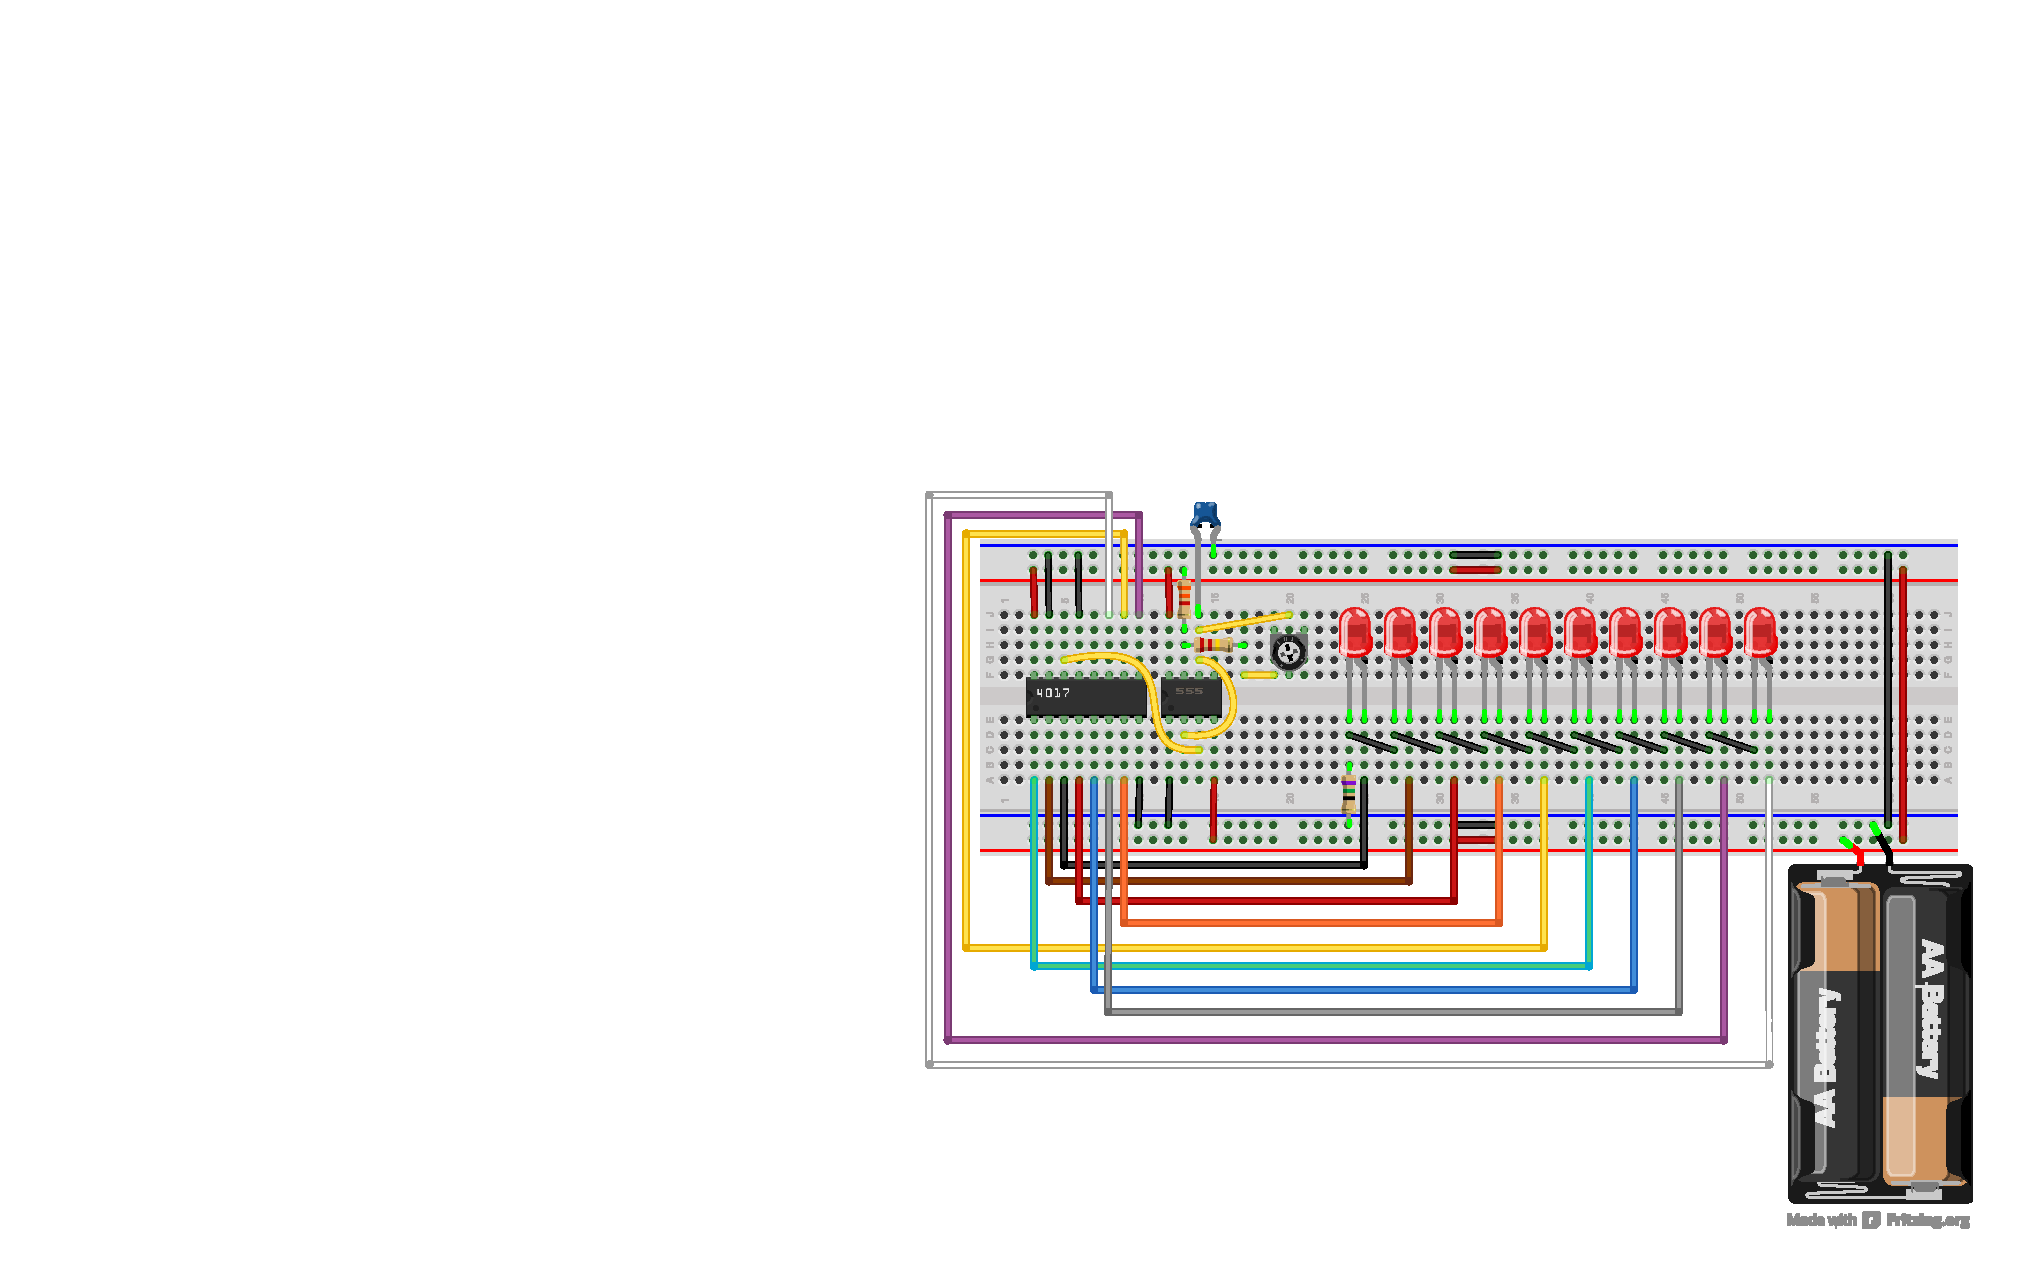
\includegraphics[width=10cm]{fig/rinnande_ljus_bb.pdf}
\end{center}
\end{figure}

\end{center}

\end{titlepage}

%%%%%%%%%%%%%%%%%%%% Header %%%%%%%%%%%%%%%%%%%%%%%%
\pagestyle{empty}
\fancyhead[l]{Nybörjarkit: Rinnande ljus}
\fancyhead[r]{Albert Skog, \today}
%%%%%%%%%%%%%%%%%% Innehåll %%%%%%%%%%%%%%%%%%%%%%%

\tableofcontents
\clearpage
\pagestyle{fancy}
\setcounter{page}{1}
\section{Inledning}
Sedan urminnes tider (1962) har blinkande lysdioder förundrat och belyst aspirerande elektronikingenjörer. Det här dokumentet beskriver hur man enkelt konstruerar en respektingivande rinnande-ljus-krets som passar till både vardag och fest. Det här dokumentet beskriver \textbf{inte} hur man löder -- för information om det, fråga någon som vet.

\section{Konstruktion}
\emph{Det här är kapitlet om hur kretsen fungerar. Om du bara vill bygga den så kan du hoppa över det så länge.}\\

Det finns så klart oändligt många metoder ($metoder\rightarrow \infty$)  för att tända lysdioder en i taget. Ett enkelt och vanligt sätt är att använda dekadräknaren \emph{4017}. Den har mycket lämpliga egenskaper för ändamålet; tio utgångar som aktiveras en i taget med hjälp av en klocksignal. De tio utgångarna kan dessutom leverera tillräckligt med ström för att driva lysdioder, vilket inte alltid är fallet med IC-kretsar. I figur \ref{fig:sch} kan vi se att allt som 4017 behöver är strömförsörjning och pulserna från 555:an som bestämmer hur fort ljuset ska rinna. Det finns många olika sätt att generera pulser till 4017:s klockingång. \emph{555} är ett mycket vanligt timerchip som går att använda på många olika sätt. I denna konfiguration genererar den en fyrkantsvåg med lika långa ettor som nollor. Om du vill generera en enda puls, eller göra korta pulser med långa mellanrum så går det också att göra om man kopplar in kringkomponenterna annorlunda.

\begin{figure}[h]
\centering
\fbox{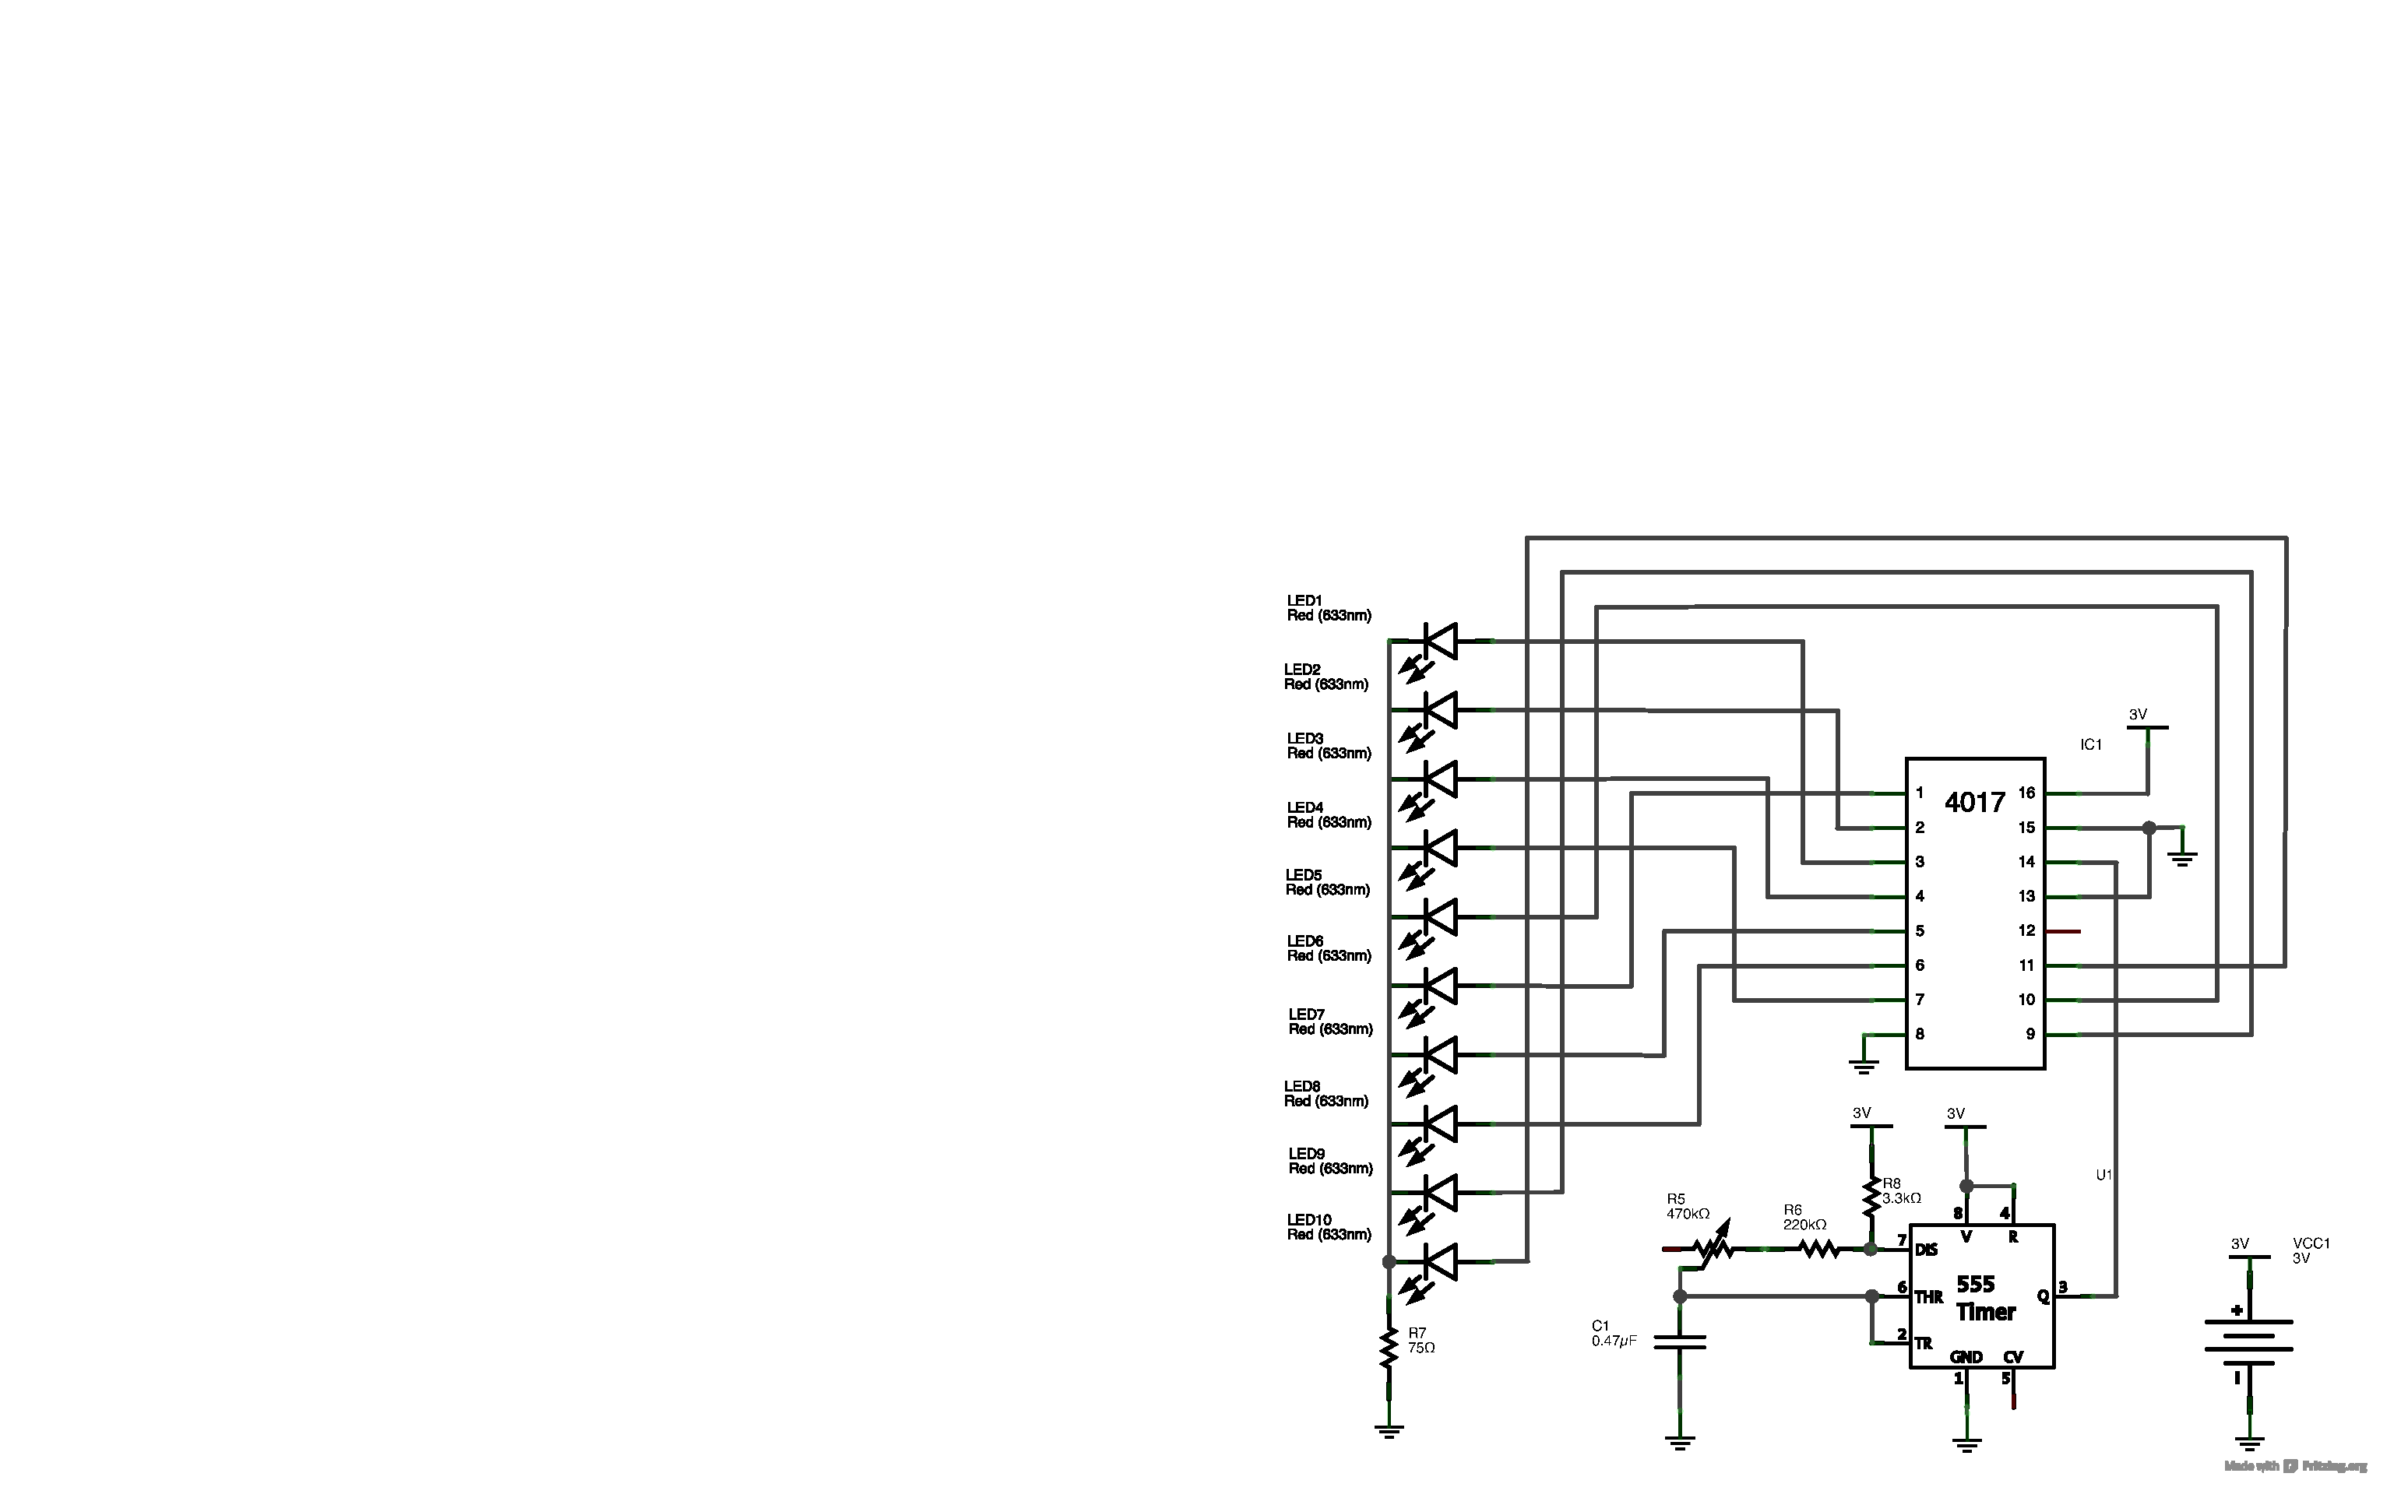
\includegraphics[width=12cm]{fig/rinnande_ljus_schem.pdf}}
\caption{Kopplingsschema.}
\label{fig:sch}
\end{figure}


\begin{wrapfigure}{r}{0.3\textwidth}
\vspace{-10pt}
\centering
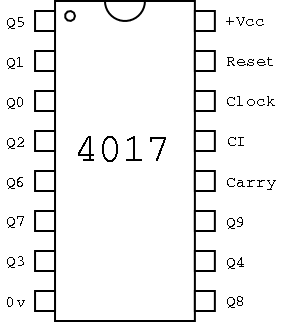
\includegraphics[width=3cm]{fig/4017.png}
\caption{Pinout för 4017.}
\label{fig:4017}
\end{wrapfigure}

\subsection{Räknare 4017}

Det finns uppskattningsvis $4 \cdot 10^{13}$ olika sorters chip i världen. Några av dem ingår i 4000-serien som introducerades 1968 som en uppföljare till den klassiska 74-serien. Just 4017 är en räknare som räknar klockpulser. Man kan tänka sig att lysdioderna i vår krets representerar ett binärt tal, den "rinnande" sekvensen skulle då motsvara $2^0, 2^1, 2^2, 2^3$ och så vidare (därav namnet dekadräknare).

I figur \ref{fig:4017} visas benämningarna för alla chipets in- och utgångar. Notera att \emph{reset} kopplats till jord, om den hade lämnats flytande kunde statisk elektricitet eller liknande ha startat om räknaren oväntat. Utgångarna \emph{carry} och \emph{CI} används inte i vårt projekt, men behövs om man till exempel vill koppla samman flera räknare.

\subsection{Timer 555}
555 är en mycket välkänd och mångsidig timer. Den kan konfigureras på en rad olika sätt; den kan generera pulser av en viss längd när en knapp trycks ned generera asymmetriska eller, som i vårat fall, symmetriska fyrkantsvågor för att nämna några.

\subsection{LED1-10}
Efter att ha beskådat kopplingsschemat bör du reagerat på att alla lysdioderna är kopplade till en enda resistor. I vanliga fall ska lysdioder alltid ha egna strömbegränsningsmotstånd, men i vår krets kommer ju ändå bara en diod i taget vara tänd, så det behövs alltså inte.


\section{Guide}

Det smartaste sättet att bygga en krets är att stegvis se till att alla delar fungerar. Därför ska vi börja med att koppla upp timer-delen och se till att den fungerar, sedan lägga till räknaren.

\begin{table}[h]
\centering
\caption{Komponentlista.}
\label{tab:komp}
\begin{tabular}{l rl}
Komponent & Värde\\
\hline
C1  & 0.47 & $\mu f$\\
IC1 & 4017 & \\
IC2 & 555  & \\
LED1-10 &10&$mA$\\
R5  & 470 & $k\Omega$\\
R6  & 220 & $k\Omega$\\
R7  & 75  & $\Omega$\\
R8  & 3.3 & $k\Omega$\\
\end{tabular}
\end{table}

\subsection*{Steg 1: Timer 555}
Koppla upp timer 555 enligt figur \ref{fig:555sch} nedan.

\begin{figure}[h]
\centering
\subfloat[Kopplingsschema]{\label{}\fbox{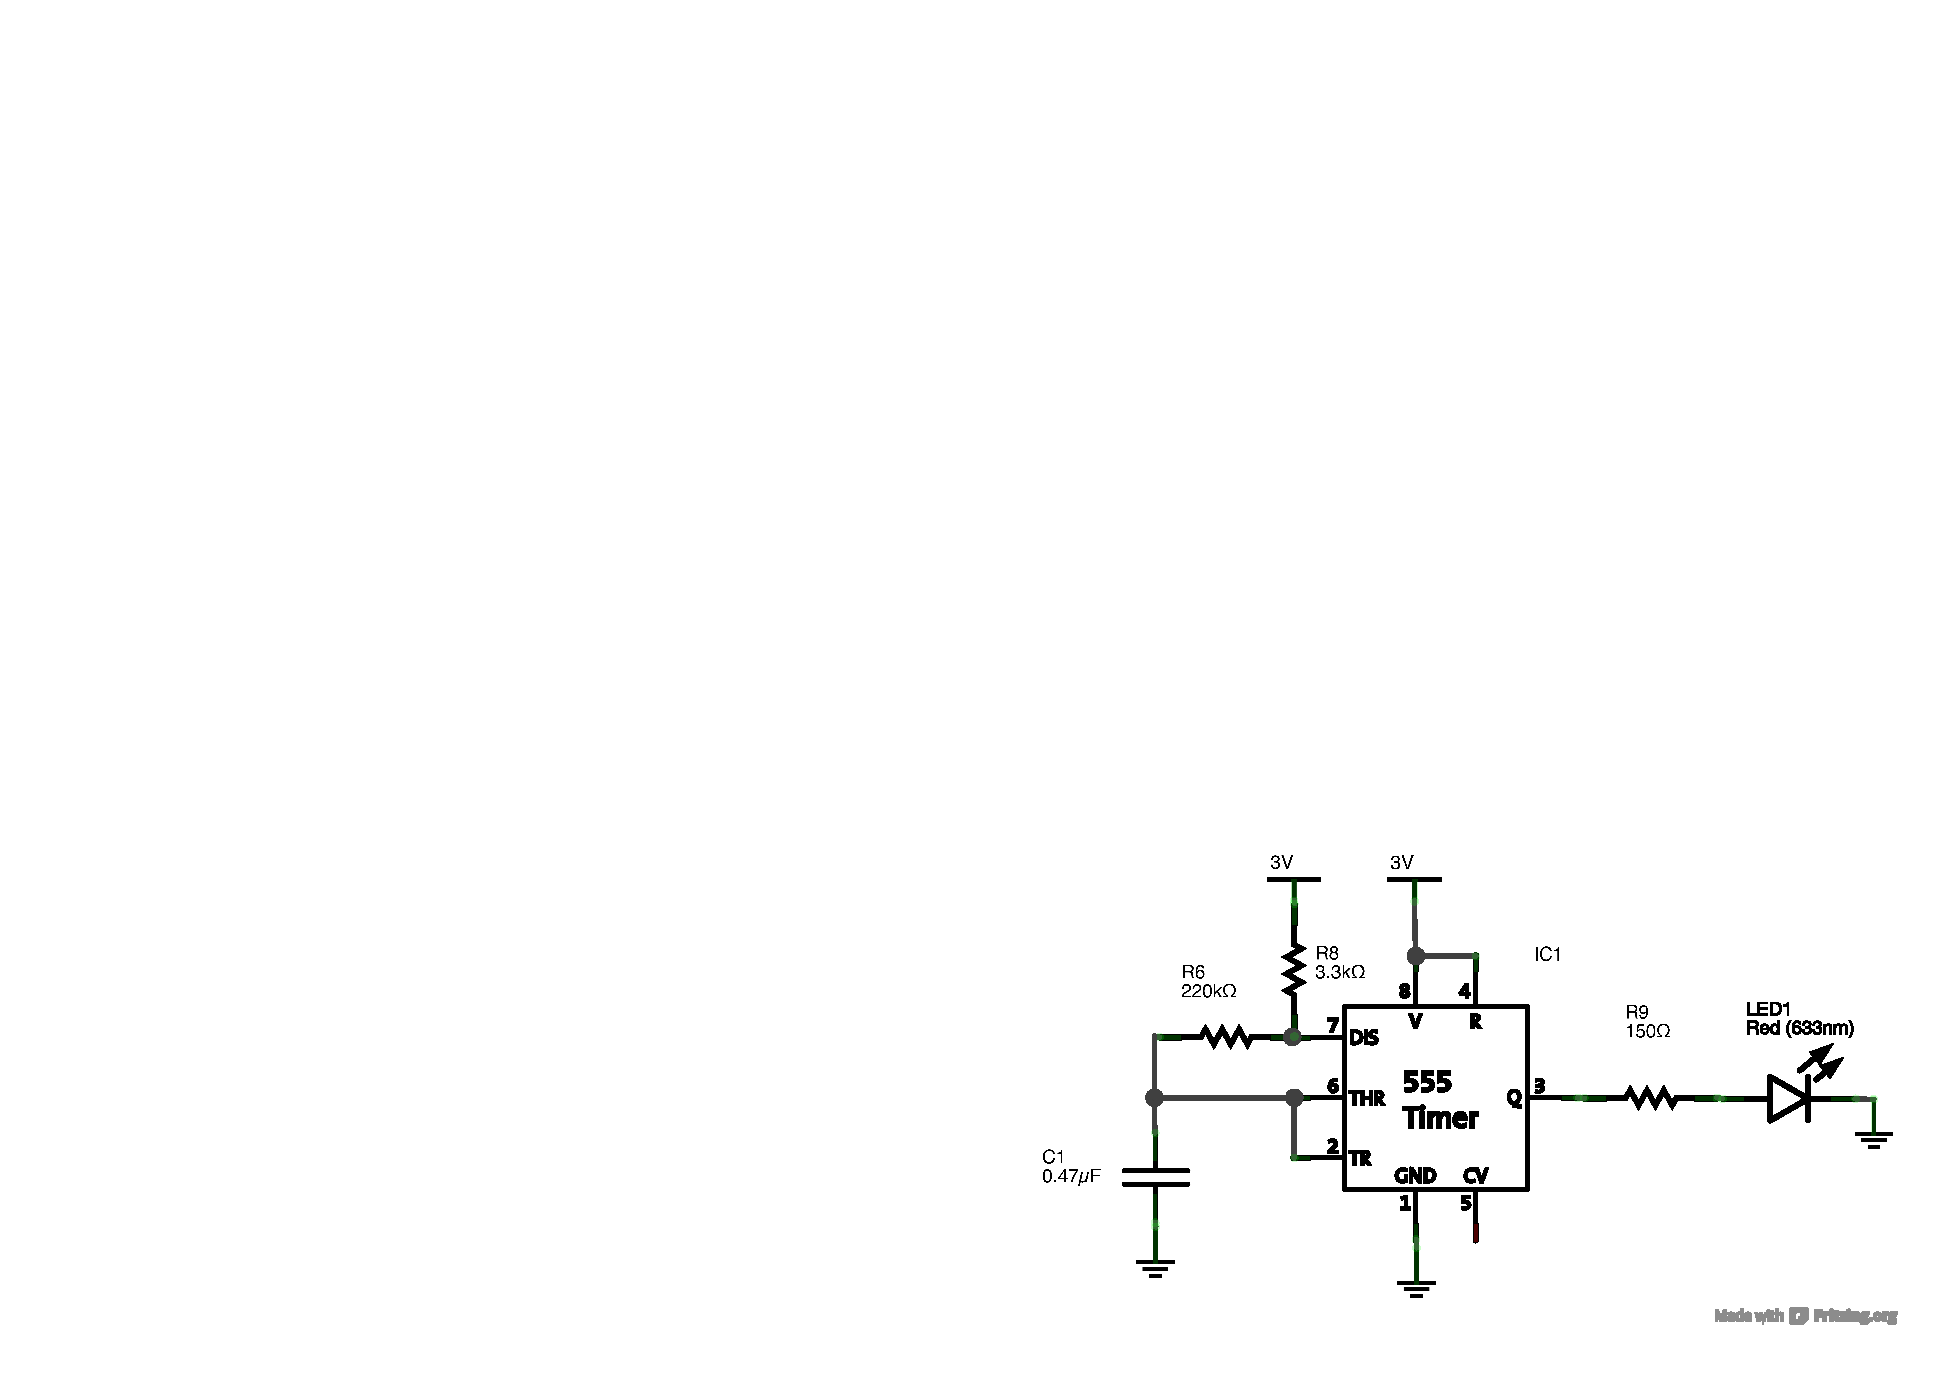
\includegraphics[height=4cm]{fig/555_test_schem.pdf}}}
\hspace{20pt}
\subfloat[Exempel på uppkoppling]{\label{}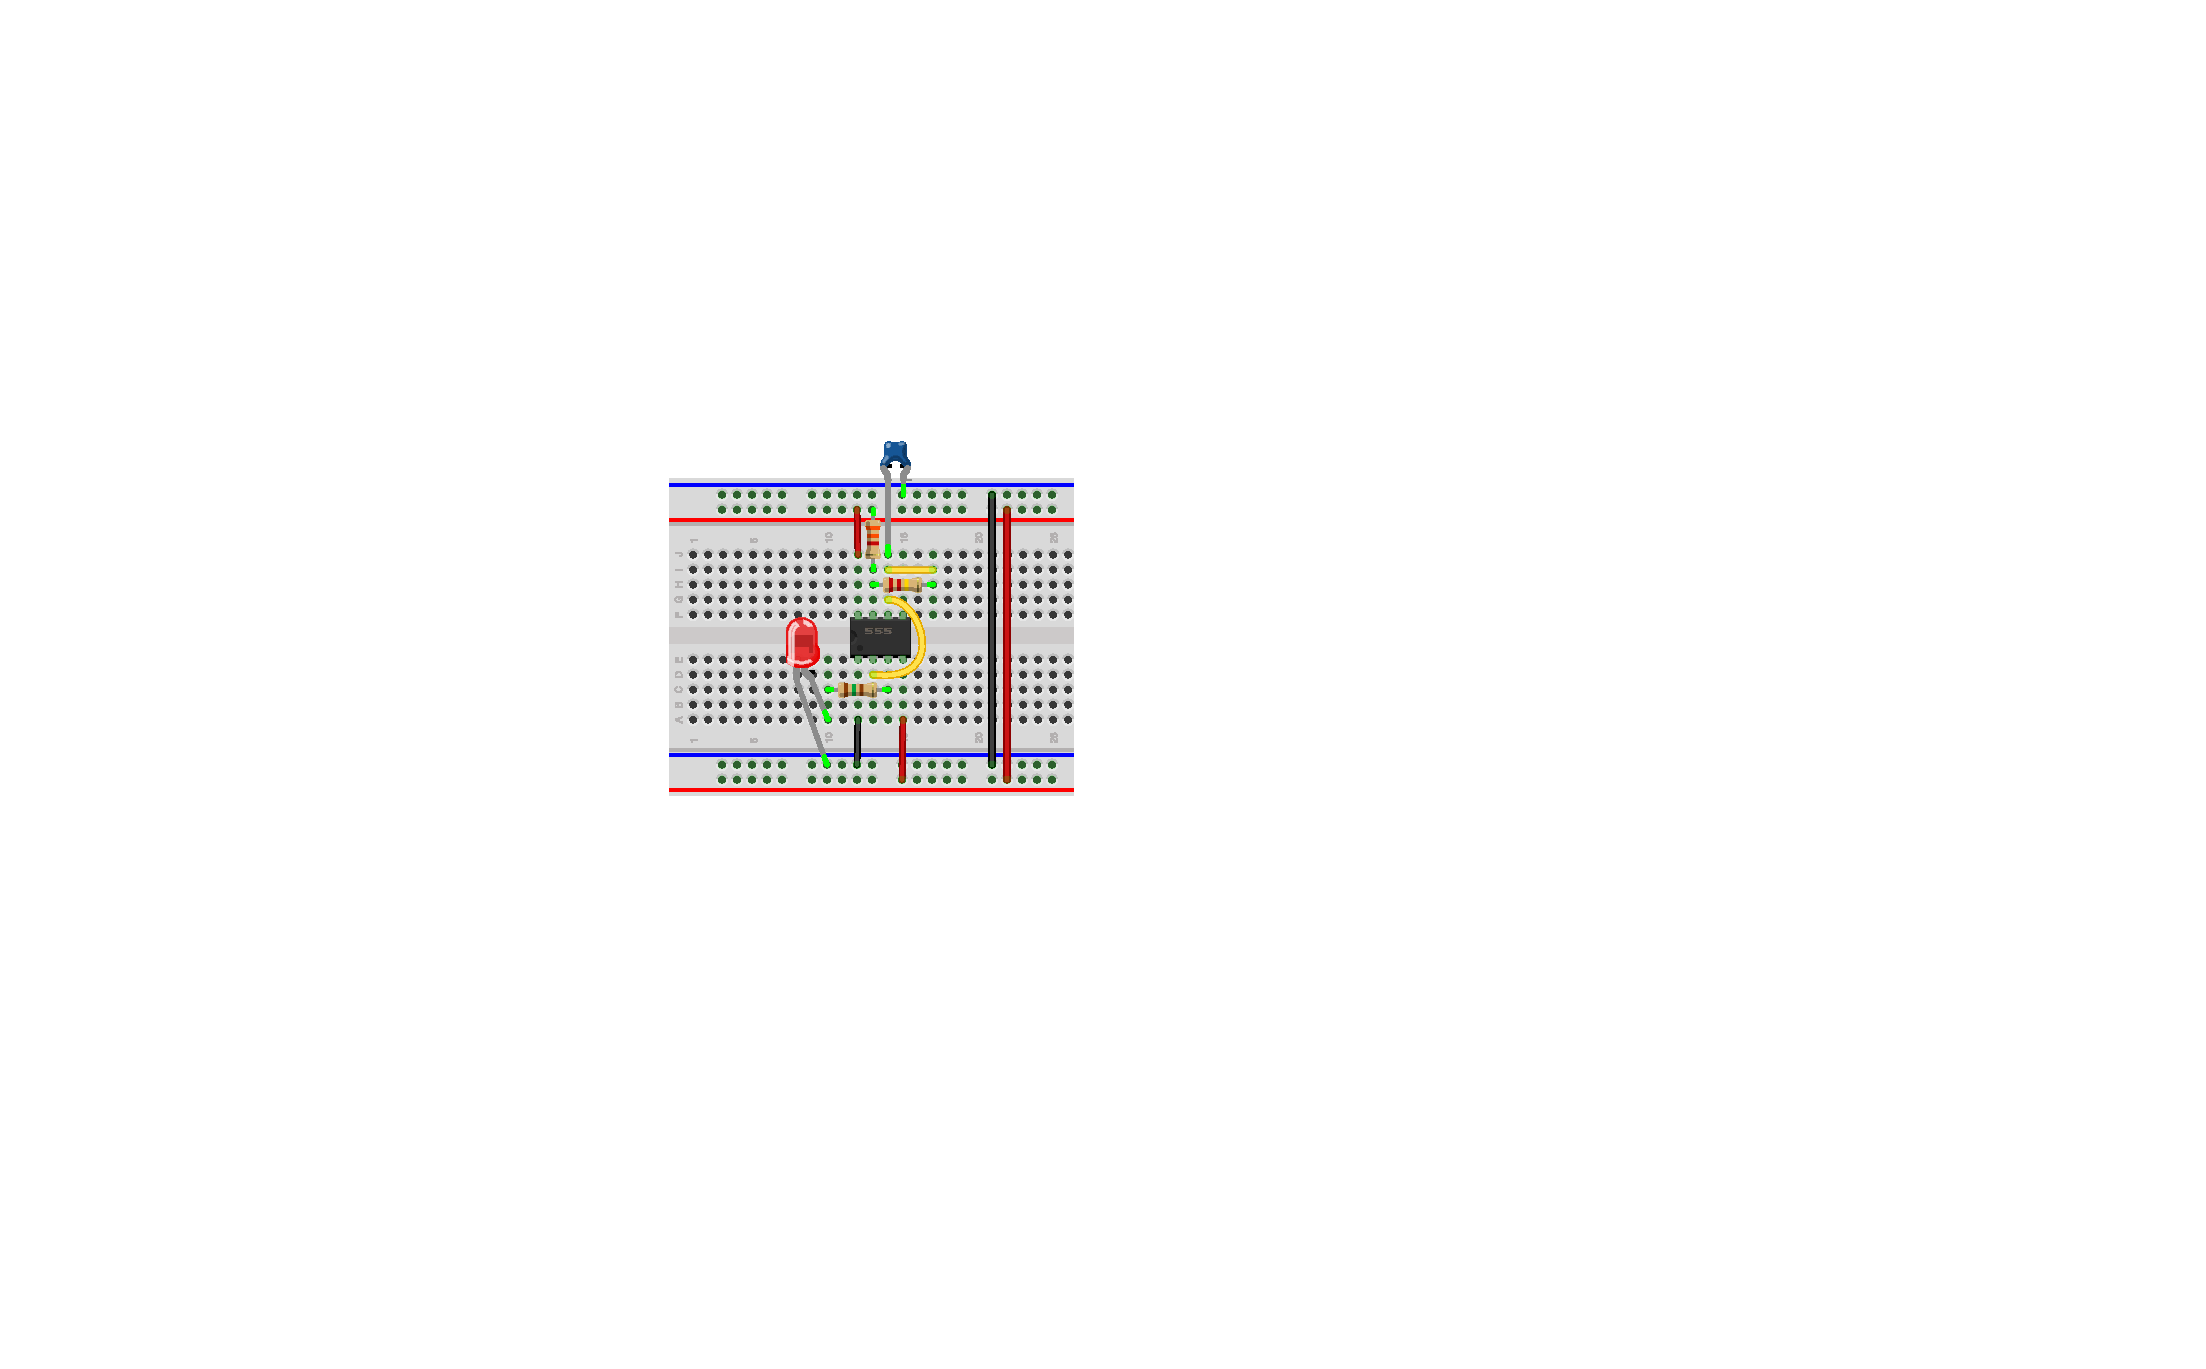
\includegraphics[height=4cm]{fig/555_test_bb.pdf}}
\caption{Test av timer 555.}
\label{fig:555sch}
\end{figure}

Kondensatorn och resistorernas värden kan ändras för att ge utsignalen en annan frekvens. För att timer 555 ska fungera rekommenderas att R1 väljs mellan $1~k\Omega$ och $1~M\Omega$ och R2 mellan $10~k\Omega$ och $1~M\Omega$. R3 är strömbegränsningsmotstånd för lysdioden och väljs till $150~\Omega$. Detta motstånd styr hur ljust lysdioden lyser och krävs för att den inte ska gå sönder. Om du vet spänningsfall ($V_d$) och maxström ($I_d$) för de lysdioder du använder kan ett mer exakt värde beräknas med Ohms lag \eqref{eq:led}.

\begin{equation}\label{eq:led}
U = R\cdot I \Leftrightarrow R = \frac{U}{I} \Leftrightarrow R = \frac{VCC-V_{d} }{I_{d}} \approx \frac{3-1.7}{10\cdot 10^{-3}} = 130~\Omega \approx 150~\Omega
\end{equation}

För att testa kretsen, koppla in en spänningsgenerator till plus- och minus och starta generatorn på 3V och med låg strömbegränsning. Det senare kan rädda dina komponenter ifall någonting är felaktigt inkopplat! Om allt är rätt borde lysdioden nu blinka ungefär tio gånger per sekund.

\subsection*{Steg 2: Räknare 4017}
Du kan nu koppla in räknaren och lysdioderna. Titta på kopplingsschemat \ref{fig:schem} och (om du vill) på kopplingsförslaget (figur \ref{fig:kopplingsplatta}).

\begin{figure}[H]
\centering
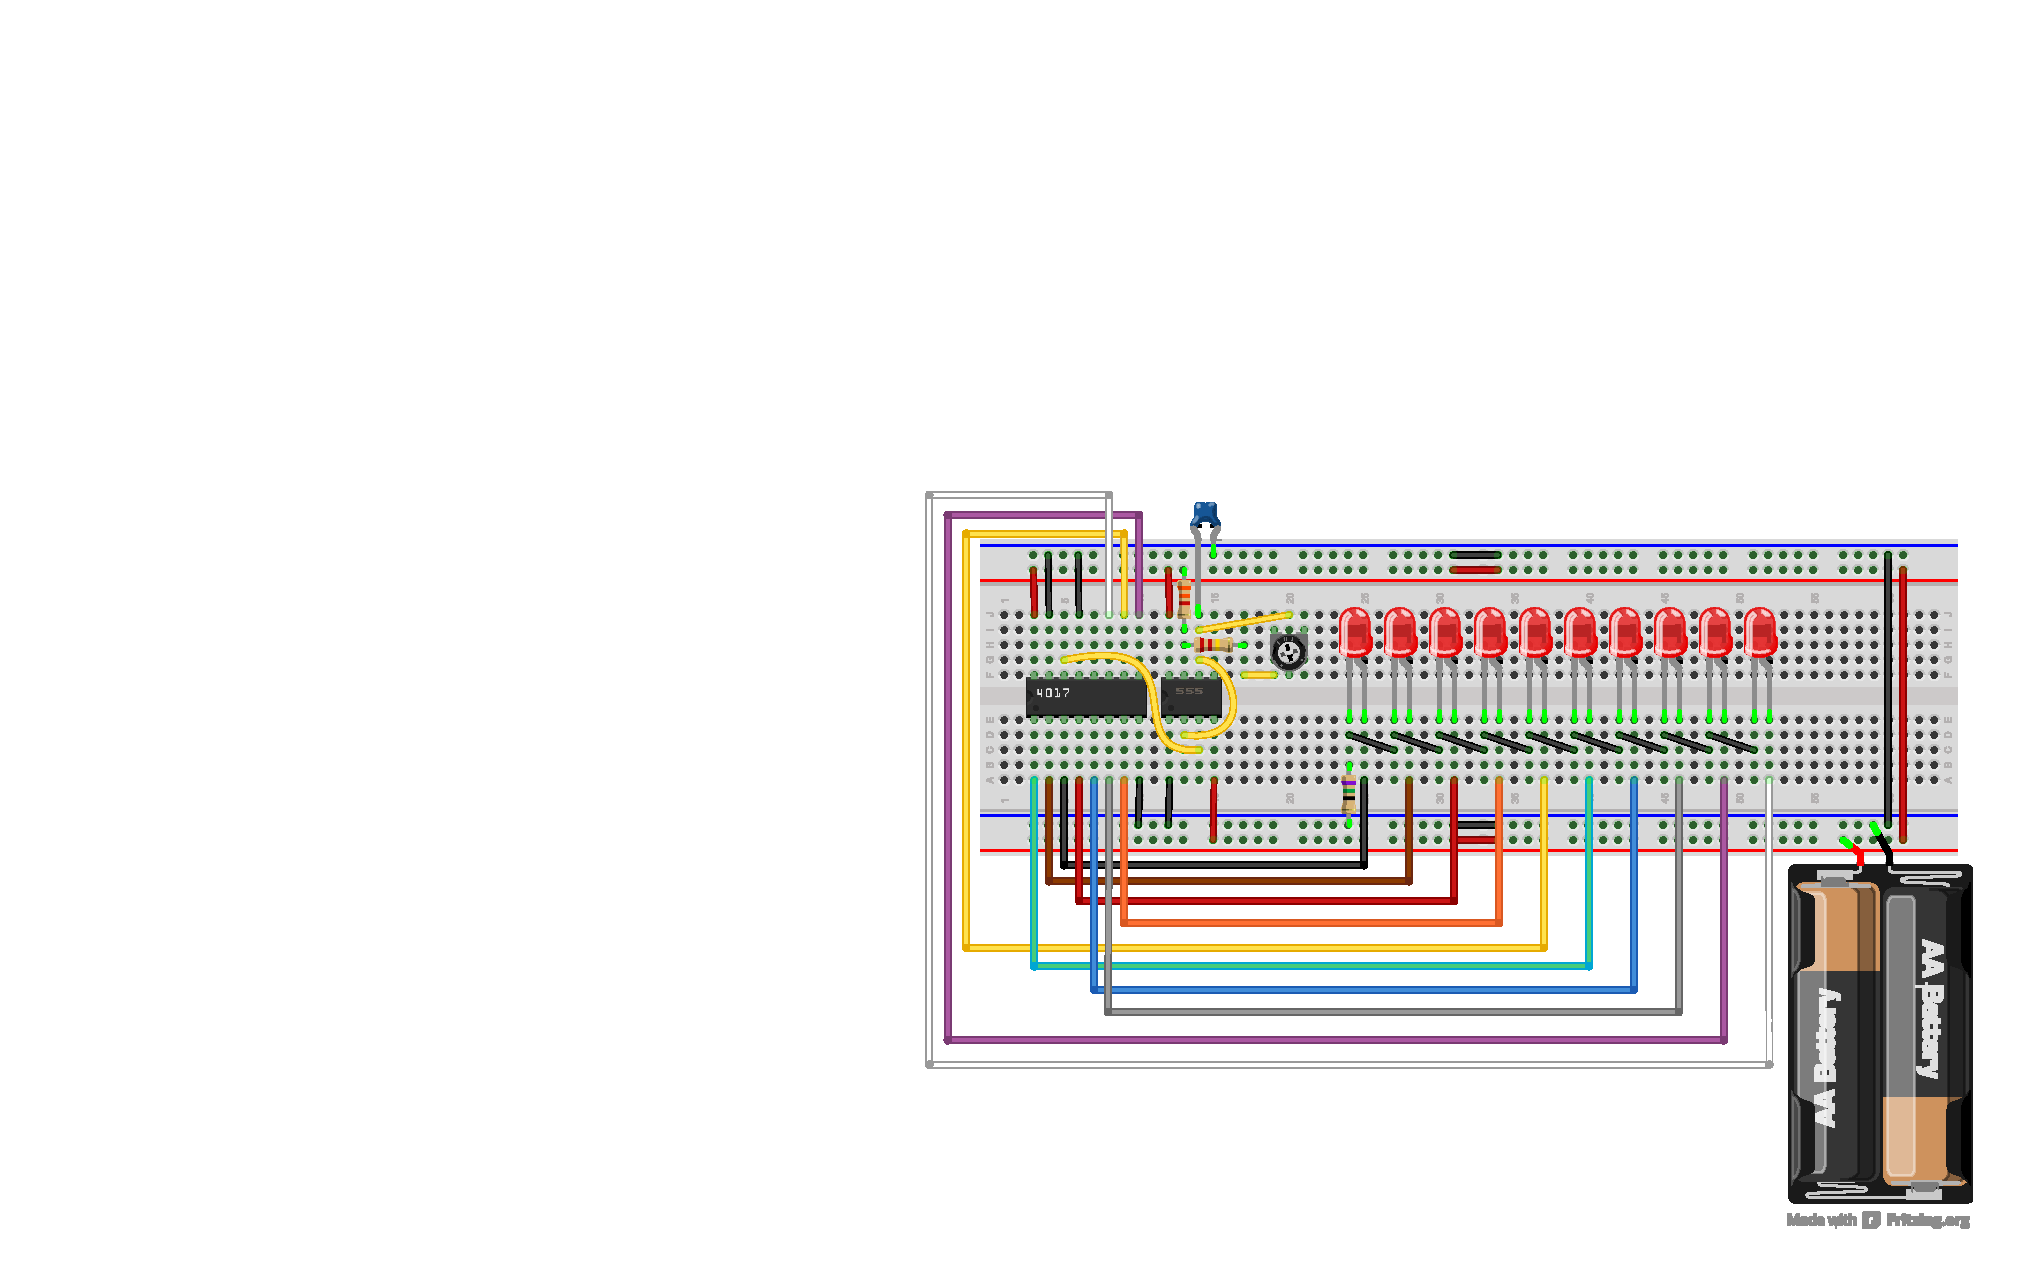
\includegraphics[width=13cm]{fig/rinnande_ljus_bb.pdf}
\caption{Ritning över kretsen uppkopplad på kopplingsplatta.}
\label{fig:kopplingsplatta}
\end{figure}

\subsection*{Steg 3: Lödning}
När du är nöjd med funktionen hos din krets kan du gå vidare och löda ihop allt på ett experimentkort. Det Finns olika typer av kort, en del har heldragna banor, andra sitter ihop tre och tre, och vissa har bara enskilda öar. Figur \ref{fig:experimentkort} visar ett möjligt sätt att löda ihop ett kort med längsgående banor. Säkerligen finns smartare och mer kompakta sätt som kräver färre sladdar.

\begin{figure}[H]
\centering
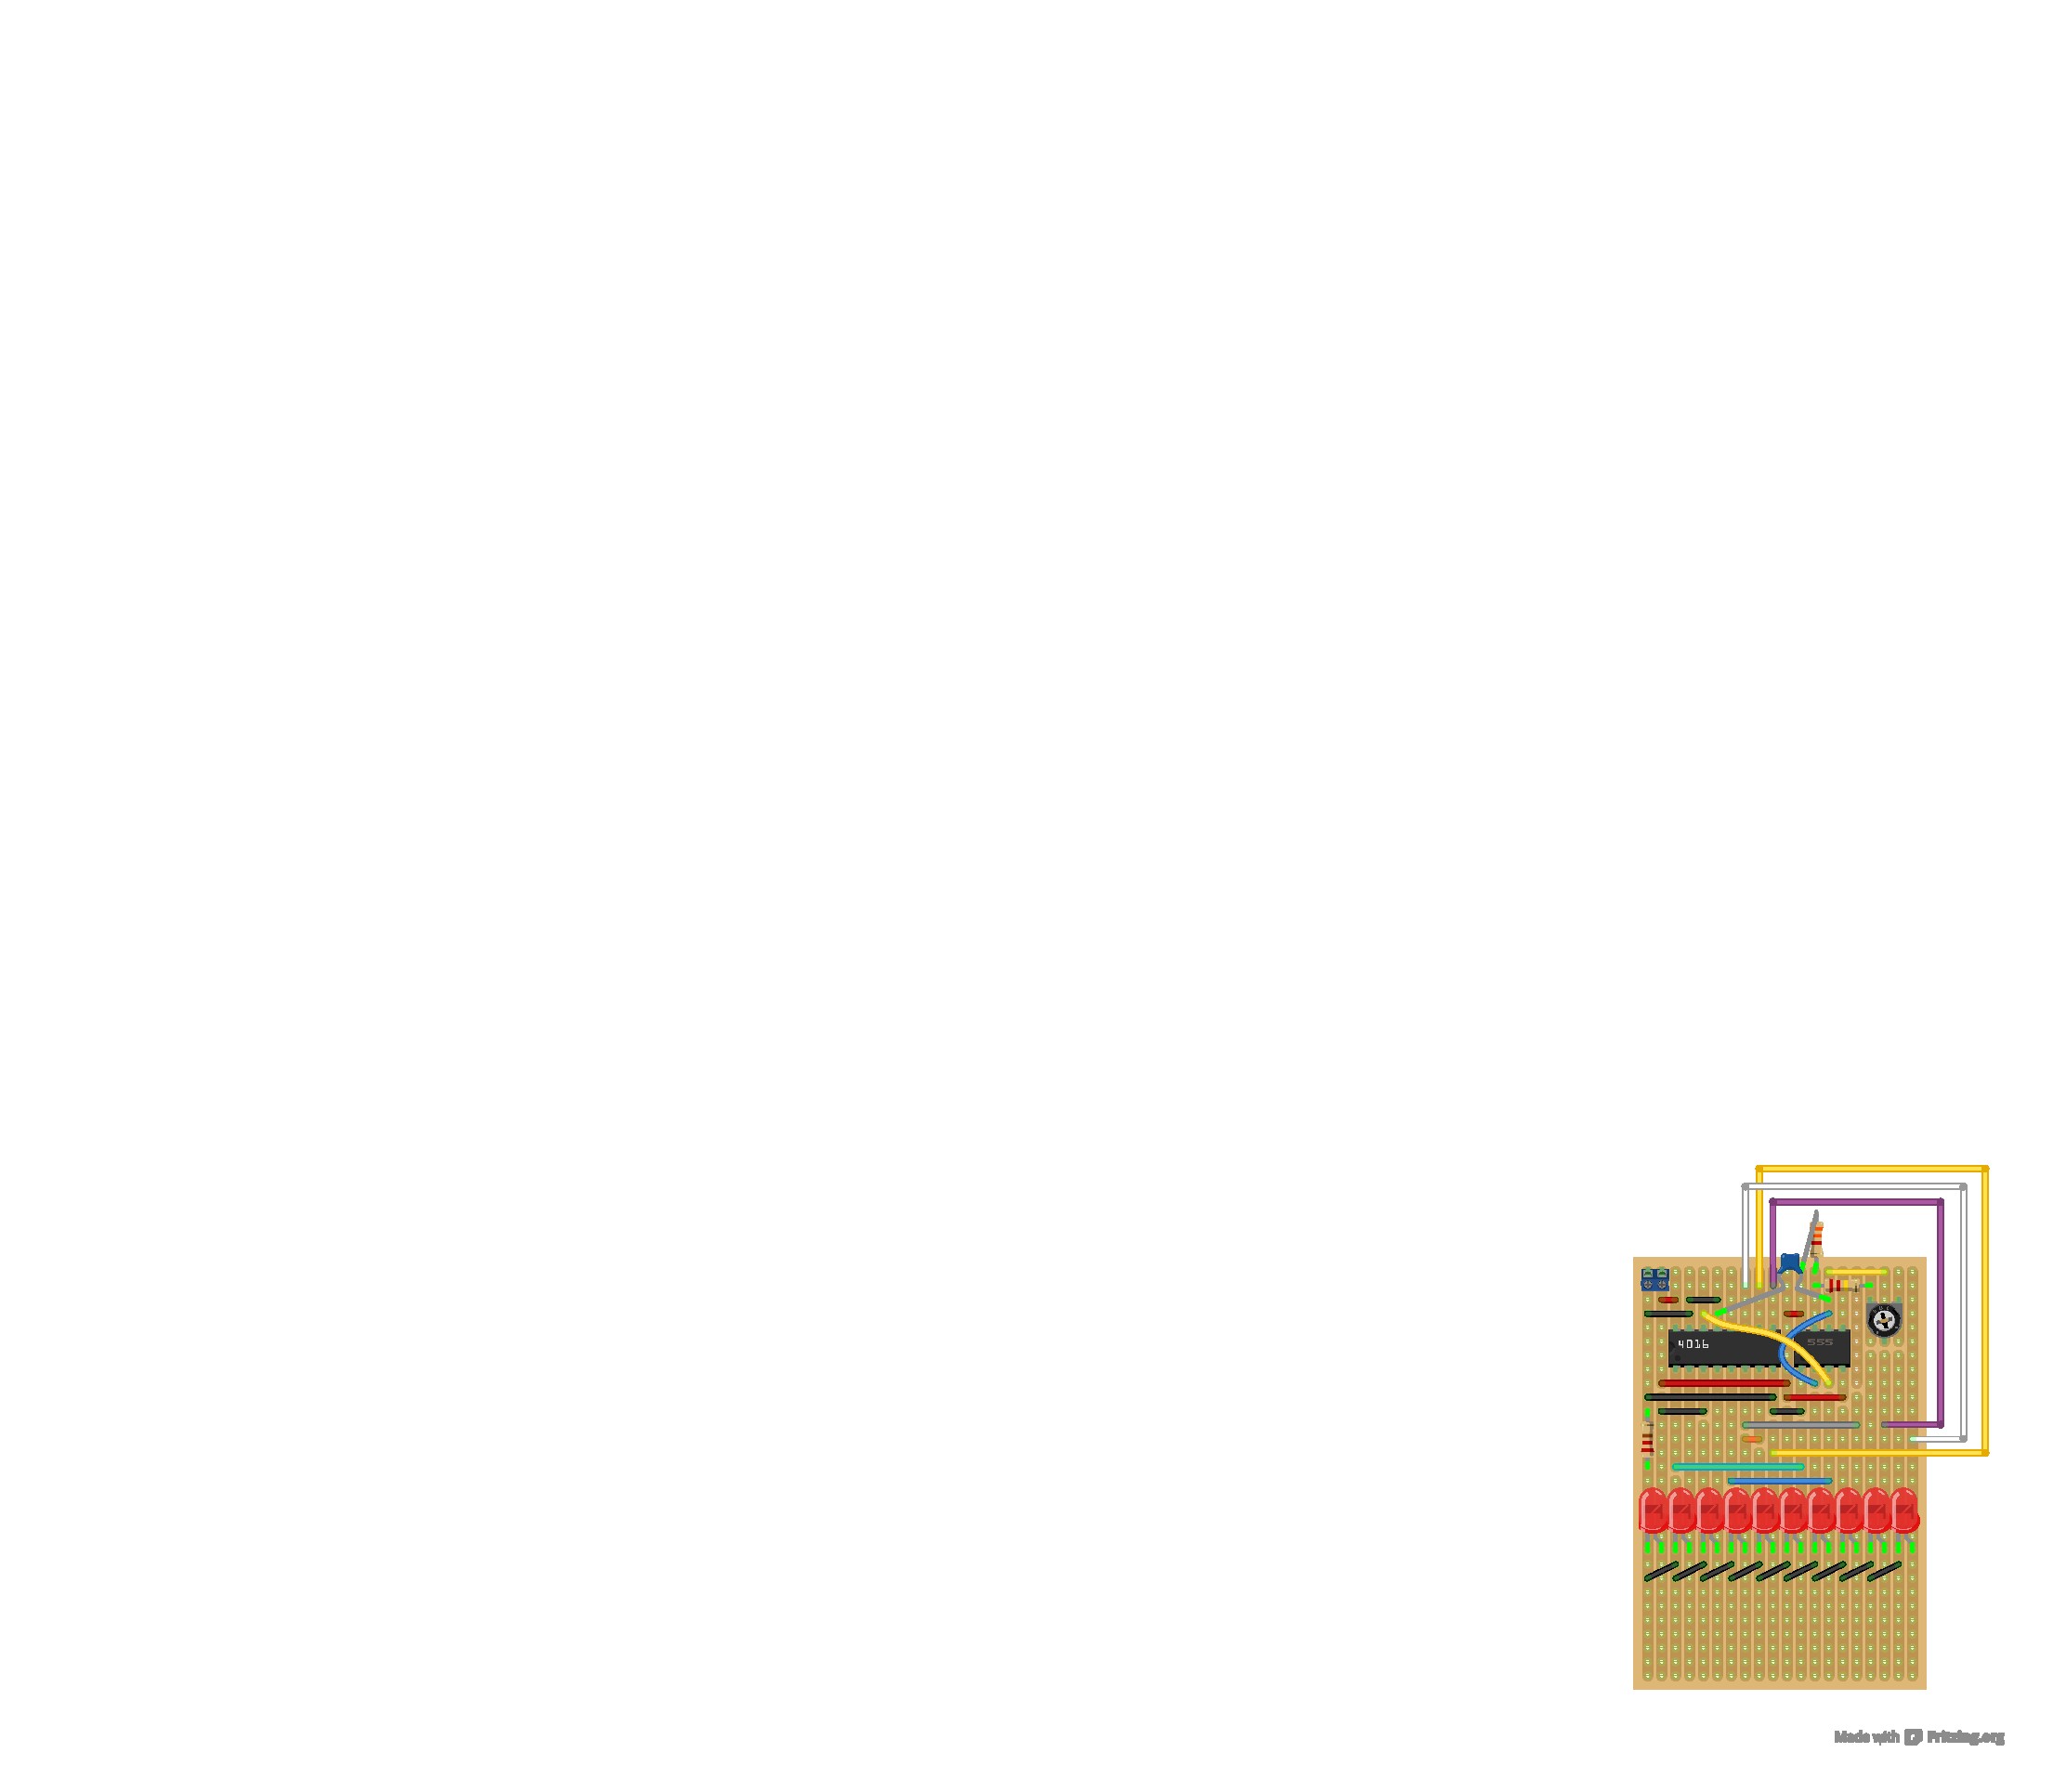
\includegraphics[width=7cm]{fig/rinnande_ljus_protoboard_bb.pdf}
\caption{}
\label{fig:experimentkort}
\end{figure}

\section{Vad ska jag göra nu?}
\begin{description}
\item[Bygg ut kretsen med en till 4017.] Det går att "haka på" en till 4017 och på så sätt lägga till ytterligare 10 lysdioder. Alternativt kan man (om man skyddar alla utgångarna med dioder) få lyset att gå fram och tillbaka. Kolla i databladet!
\item[Bygg en robot.] Låna/köp en Arduino eller en Launchpad och kolla in lite kodexempel. Det är enkelt!
\item[Lär dig \LaTeX.] Det här dokumentet är skrivet i \LaTeX, det nördigaste och i särklass coolaste sättet att skriva rapporter.
\item[Lär dig Git.]  
\end{description}

\end{document}